
\section{Bedienoberfläche}

Hier werden die Skizzen/Prototypen von der Bedienoberfläche dargestellt, als auch die Zusammenhänge zwischen denen.

\newcounter{gui}\setcounter{gui}{10}

\begin{description}[leftmargin=5em, style=sameline]	
	\begin{lhp}{gui}{GUI}{gui:beispiel}
		\item[Name:] Zusammenhänge
		\item[Beschreibung:] Zusammenhänge zwischen GUI-Ansichten
		\item[Relevante Systemfunktionen:] Alle
		\item[Abbildungen:] \ref{gui:zusammenhang}
	\end{lhp}
\end{description}

\begin{description}[leftmargin=5em, style=sameline]	
	\begin{lhp}{gui}{GUI}{gui:beispiel}
		\item[Name:] Login-Seite
		\item[Beschreibung:] Interface für Anmeldung
		\item[Relevante Systemfunktionen:] \ref{funk:zugriff}
		\item[Abbildungen:] \ref{gui:login}
	\end{lhp}
\end{description}

\begin{description}[leftmargin=5em, style=sameline]	
	\begin{lhp}{gui}{GUI}{gui:beispiel}
		\item[Name:] Registration-Seite
		\item[Beschreibung:] Interface für Registration
		\item[Relevante Systemfunktionen:] \ref{funk:zugriff}
		\item[Abbildungen:] \ref{gui:registration}
	\end{lhp}
\end{description}

\begin{description}[leftmargin=5em, style=sameline]	
	\begin{lhp}{gui}{GUI}{gui:beispiel}
		\item[Name:] Lobby Seite
		\item[Beschreibung:] Gibt Zugriff auf Raumerstellung und Beitritt, Bestenliste und Chat 
		\item[Relevante Systemfunktionen:] \ref{funk:zugriff}
		\item[Abbildungen:] \ref{gui:lobby}
	\end{lhp}
\end{description}

\begin{description}[leftmargin=5em, style=sameline]	
	\begin{lhp}{gui}{GUI}{gui:beispiel}
		\item[Name:] Spielraum-Erstellungs-Seite
		\item[Beschreibung:] Erlaubt es einem Nutzer einen Spielraum zu erstellen, optional mit einem Passwort
		\item[Relevante Systemfunktionen:] \ref{funk:zugriff}
		\item[Abbildungen:] \ref{gui:create_gameroom}
	\end{lhp}
\end{description}

\begin{description}[leftmargin=5em, style=sameline]	
	\begin{lhp}{gui}{GUI}{gui:beispiel}
		\item[Name:] Spielraumbetritt per Code Seite
		\item[Beschreibung:] Erlaubt es einem Nutzer einem Spielraum per Code beizutreten
		\item[Relevante Systemfunktionen:] \ref{funk:zugriff}
		\item[Abbildungen:] \ref{gui:join_code}
	\end{lhp}
\end{description}

\begin{description}[leftmargin=5em, style=sameline]	
	\begin{lhp}{gui}{GUI}{gui:beispiel}
		\item[Name:] Profil löschen Seite
		\item[Beschreibung:] Erlaubt es dem Nutzer sein Profil zu löschen
		\item[Relevante Systemfunktionen:] \ref{funk:zugriff}
		\item[Abbildungen:] \ref{gui:delete_prof}
	\end{lhp}
\end{description}

\begin{description}[leftmargin=5em, style=sameline]	
	\begin{lhp}{gui}{GUI}{gui:beispiel}
		\item[Name:] Spielraum-Seite
		\item[Beschreibung:] Gibt Zugriff auf den Ready-Check um das Spiel zu starten, als auch dem Besitzer Spieler zu entfernen und Bots hinzuzufügen und zu entfernen
		\item[Relevante Systemfunktionen:] \ref{funk:zugriff}
		\item[Abbildungen:] \ref{gui:gameroom}
	\end{lhp}
\end{description}

\begin{description}[leftmargin=5em, style=sameline]	
	\begin{lhp}{gui}{GUI}{gui:beispiel}
		\item[Name:] Spielbrett-Seite
		\item[Beschreibung:] Zeigt das Spielbrett, als auch wahlweise den Game- und Globalchat
		\item[Relevante Systemfunktionen:] \ref{funk:zugriff}
		\item[Abbildungen:] \ref{gui:gameboard}
	\end{lhp}
\end{description}

\begin{description}[leftmargin=5em, style=sameline]	
	\begin{lhp}{gui}{GUI}{gui:beispiel}
		\item[Name:] Spielende-Seite
		\item[Beschreibung:] Wird nach dem Spielende gezeigt und verkündet den Sieger und den Punktestand 
		\item[Relevante Systemfunktionen:] \ref{funk:zugriff}
		\item[Abbildungen:] \ref{gui:win}
	\end{lhp}
\end{description}

\begin{figure}[!h]
	\centering
	\includegraphics[width=0.9\textwidth]{SEP_Lasten_Pflichtenheft/img/Übergangsdiagramm(2).png}
	\caption{Die Zusammenhänge zwischen GUI-Ansichten.}
	\label{gui:zusammenhang}
\end{figure}

\begin{figure}[!h]
	\centering
	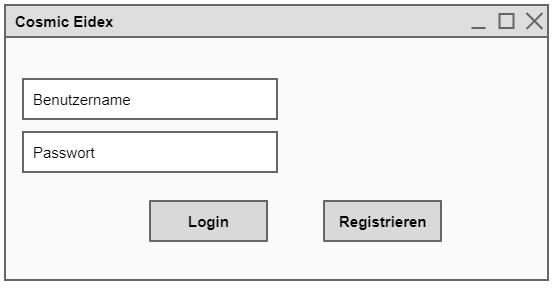
\includegraphics[width = 0.9\textwidth]{SEP_Lasten_Pflichtenheft/img/login_screen.png}
	\caption{Login-Seite}
	\label{gui:login}
\end{figure}

\begin{figure}[!h]
	\centering
	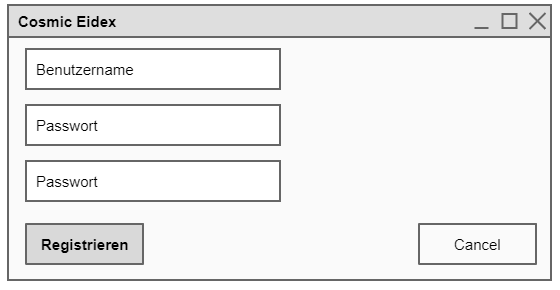
\includegraphics[width = 0.9\textwidth]{SEP_Lasten_Pflichtenheft/img/Registration Screen.png}
	\caption{Registration-Seite}
	\label{gui:registration}
\end{figure}

\begin{figure}[!h]
	\centering
	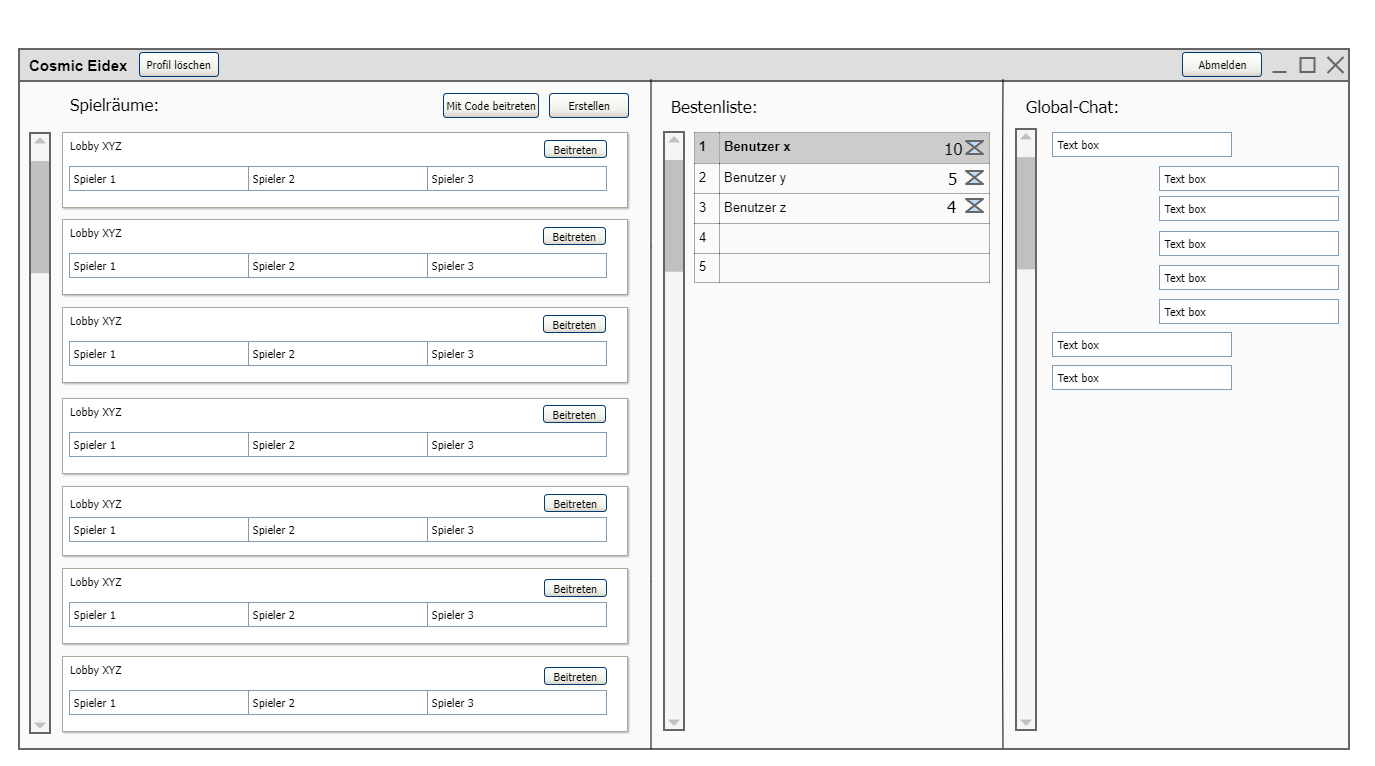
\includegraphics[width = 0.9\textwidth]{SEP_Lasten_Pflichtenheft/img/Looby Screen.png}
	\caption{Lobby-Seite}
	\label{gui:lobby}
\end{figure}

\begin{figure}[!h]
	\centering
	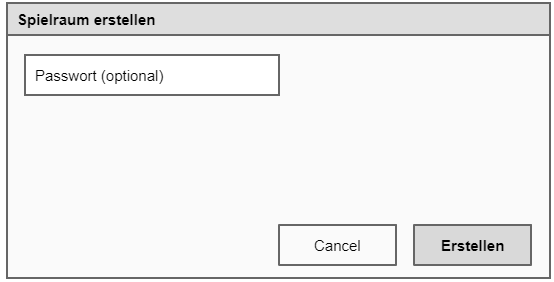
\includegraphics[width = 0.9\textwidth]{SEP_Lasten_Pflichtenheft/img/erstellen.png}
	\caption{Spielraum-Erstellungs-Seite}
	\label{gui:create_gameroom}
\end{figure}

\begin{figure}[!h]
	\centering
	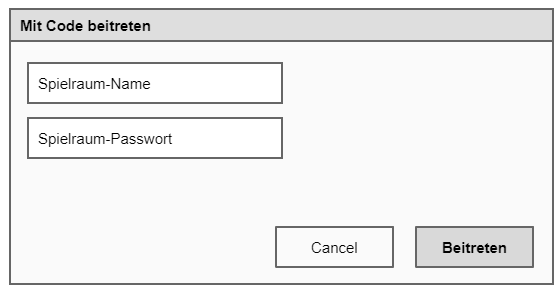
\includegraphics[width = 0.9\textwidth]{SEP_Lasten_Pflichtenheft/img/Mit Code Beitreten.png}
	\caption{Spielraumbeitritt per Code Seite}
	\label{gui:join_code}
\end{figure}

\begin{figure}[!h]
	\centering
	\includegraphics[width = 0.9\textwidth]{SEP_Lasten_Pflichtenheft/img/Profil löschen screen.png}
	\caption{Profil löschen Seite}
	\label{gui:delete_prof}
\end{figure}

\begin{figure}[!h]
	\centering
	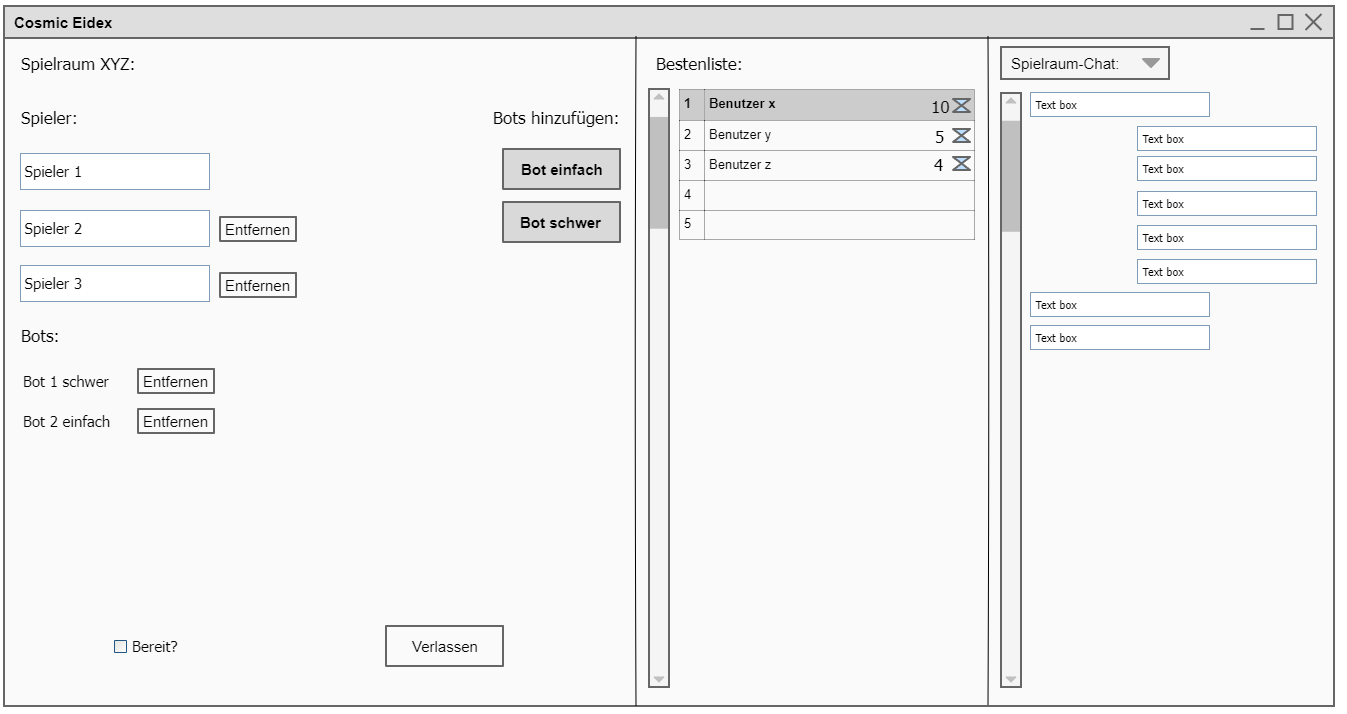
\includegraphics[width = 0.9\textwidth]{SEP_Lasten_Pflichtenheft/img/Spielraum-Screen.png}
	\caption{Spielraum-Seite}
	\label{gui:gameroom}
\end{figure}

\begin{figure}[!h]
	\centering
	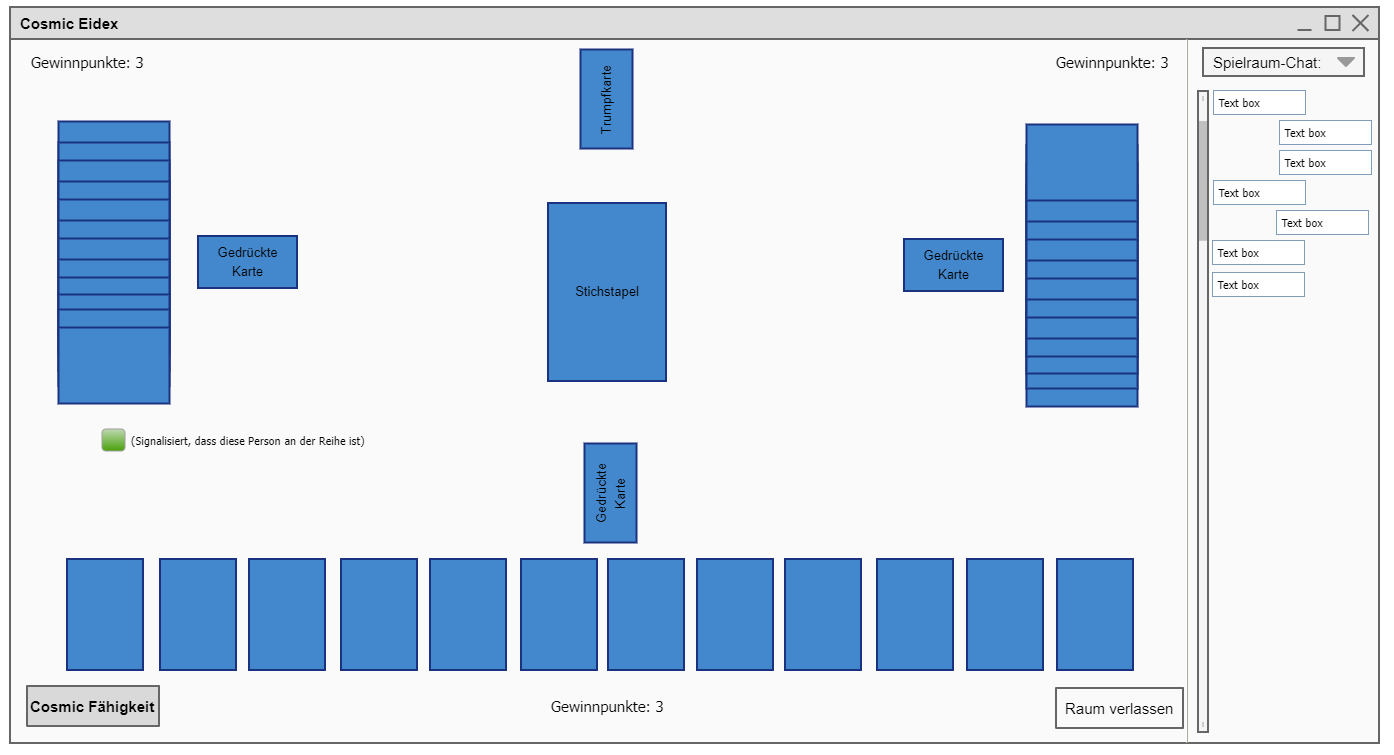
\includegraphics[width = 0.9\textwidth]{SEP_Lasten_Pflichtenheft/img/game_board_screen.png}
	\caption{Spielbrett-Seite}
	\label{gui:gameboard}
\end{figure}

\begin{figure}[!h]
	\centering
	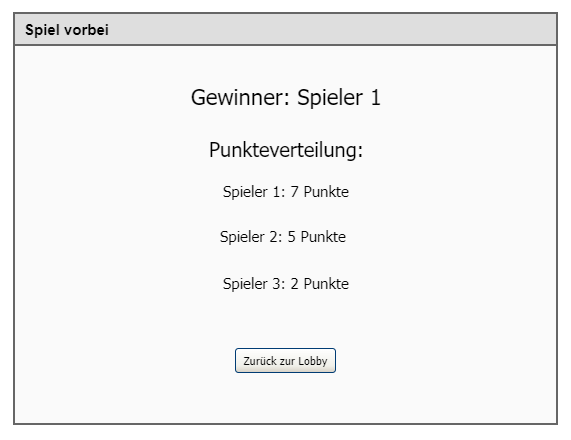
\includegraphics[width = 0.9\textwidth]{SEP_Lasten_Pflichtenheft/img/win_screen.png}
	\caption{Spielende-Seite}
	\label{gui:win}
\end{figure}